\section{Plant as sensor}

\subsection{The electronic interface}

The electronic interface is the interface that allows a compute unit to capture and interpret the plant signal and
communication. The interface is a device made by us for this use case. The printed circuit board (PCB)
device is composed of 3 main parts:
\begin{itemize}
    \item The core of the circuit, the microcontroller, an ESP32 Wroom 32
    \item An electronic filter connected using an electrode to the plant
    \item A sound part of the PCB that is including an audio amplifier, a volume knob and a terminal block to connect a speaker
\end{itemize}

The design of the PCB has been done using the open source software Kicad.
As said previously, the circuit contain 3 parts.

The core of the circuit is the computation part, including the microcontroller, an ESP32. All the other
devices of the circuit are connected to the ESP32. The choice to use a devkit has been done 
to ease the electronic conception and to avoid any communication and soldering issue with the MCU\footnote[1]{Microcontroller Unit}.

\begin{figure}[h!]
    \centering
    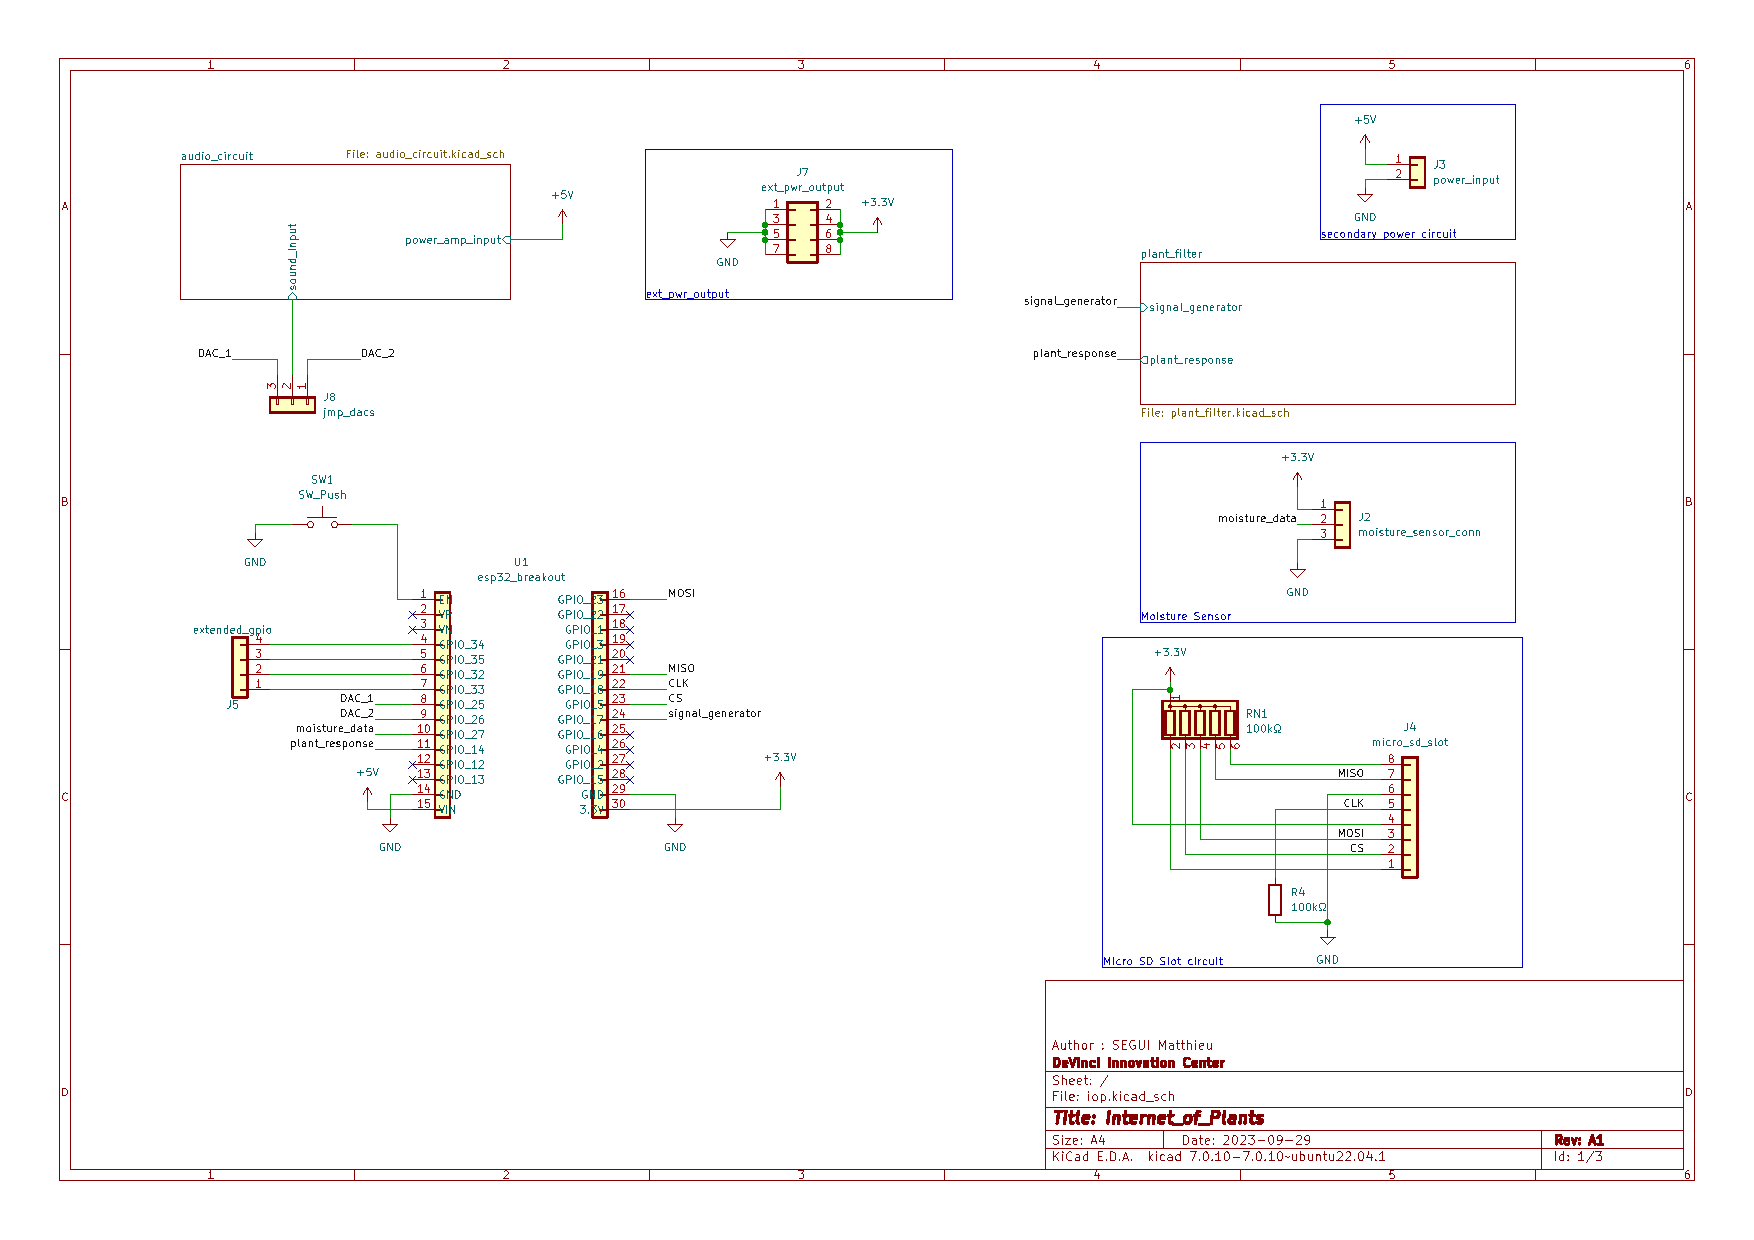
\includegraphics[width=\textwidth]{images/iop.pdf}
    \caption{The core of the circuit, the microcontroller, an ESP32 Wroom 32. All the other parts of
    circuits are plugged in.} 
    \vspace{0.1cm}
    \label{fig:iop_schematic_main}
\end{figure}

The circuit component that allows us to read data from the plant is the electronic filter.
This filter has been designed by \textit{Jakub Nikonowicz} and \textit{Łukasz Matuszewski} 
from \textit{Politechnika Poznańska}.
Thanks to them, I adapted it for my application on my embedded device. 

\begin{figure}[h!]
    \centering
    \includegraphics[width=\textwidth]{images/iop-plant_filter.pdf}
    \caption{The electronic circuit designed to capture the interaction by analyzing the electronic
    frequency response. The circuit includes 3 resistors, 3 inductors and 3 capacitors as main components} 
    \vspace{0.1cm}
    \label{fig:iop_schematic_filter}
\end{figure}

This filter is ending by a crocodile clamp that is directly connected to the plant.

The last part of the circuit is the sound output/rendering. This circuit includes a small amplifier,
the LM386 from Texas Instruments. The rest of the circuit are components needed in order to 
induce amplification on the signal without creating to many noise and saturation.

\begin{figure}[h!]
    \centering
    \includegraphics[width=\textwidth]{images/iop-audio_circuit.pdf}
    \caption{The sound output part of the circuit that is used to render the sound. 
    This part includes a small amplifier, the LM386. The circuit also includes the components necessary
    to control and handle the amplification (reduce noise and saturation)} 
    \vspace{0.1cm}
    \label{fig:iop_schematic_audio}
\end{figure}


Once the schematic is done, we have to route the tracks. It exists multiple way to route PCB 
(single-sided, double-sided, multiple layers). We choose double sided, 2 layers on each side of the PCB.

\begin{figure}[h!]
    \centering
    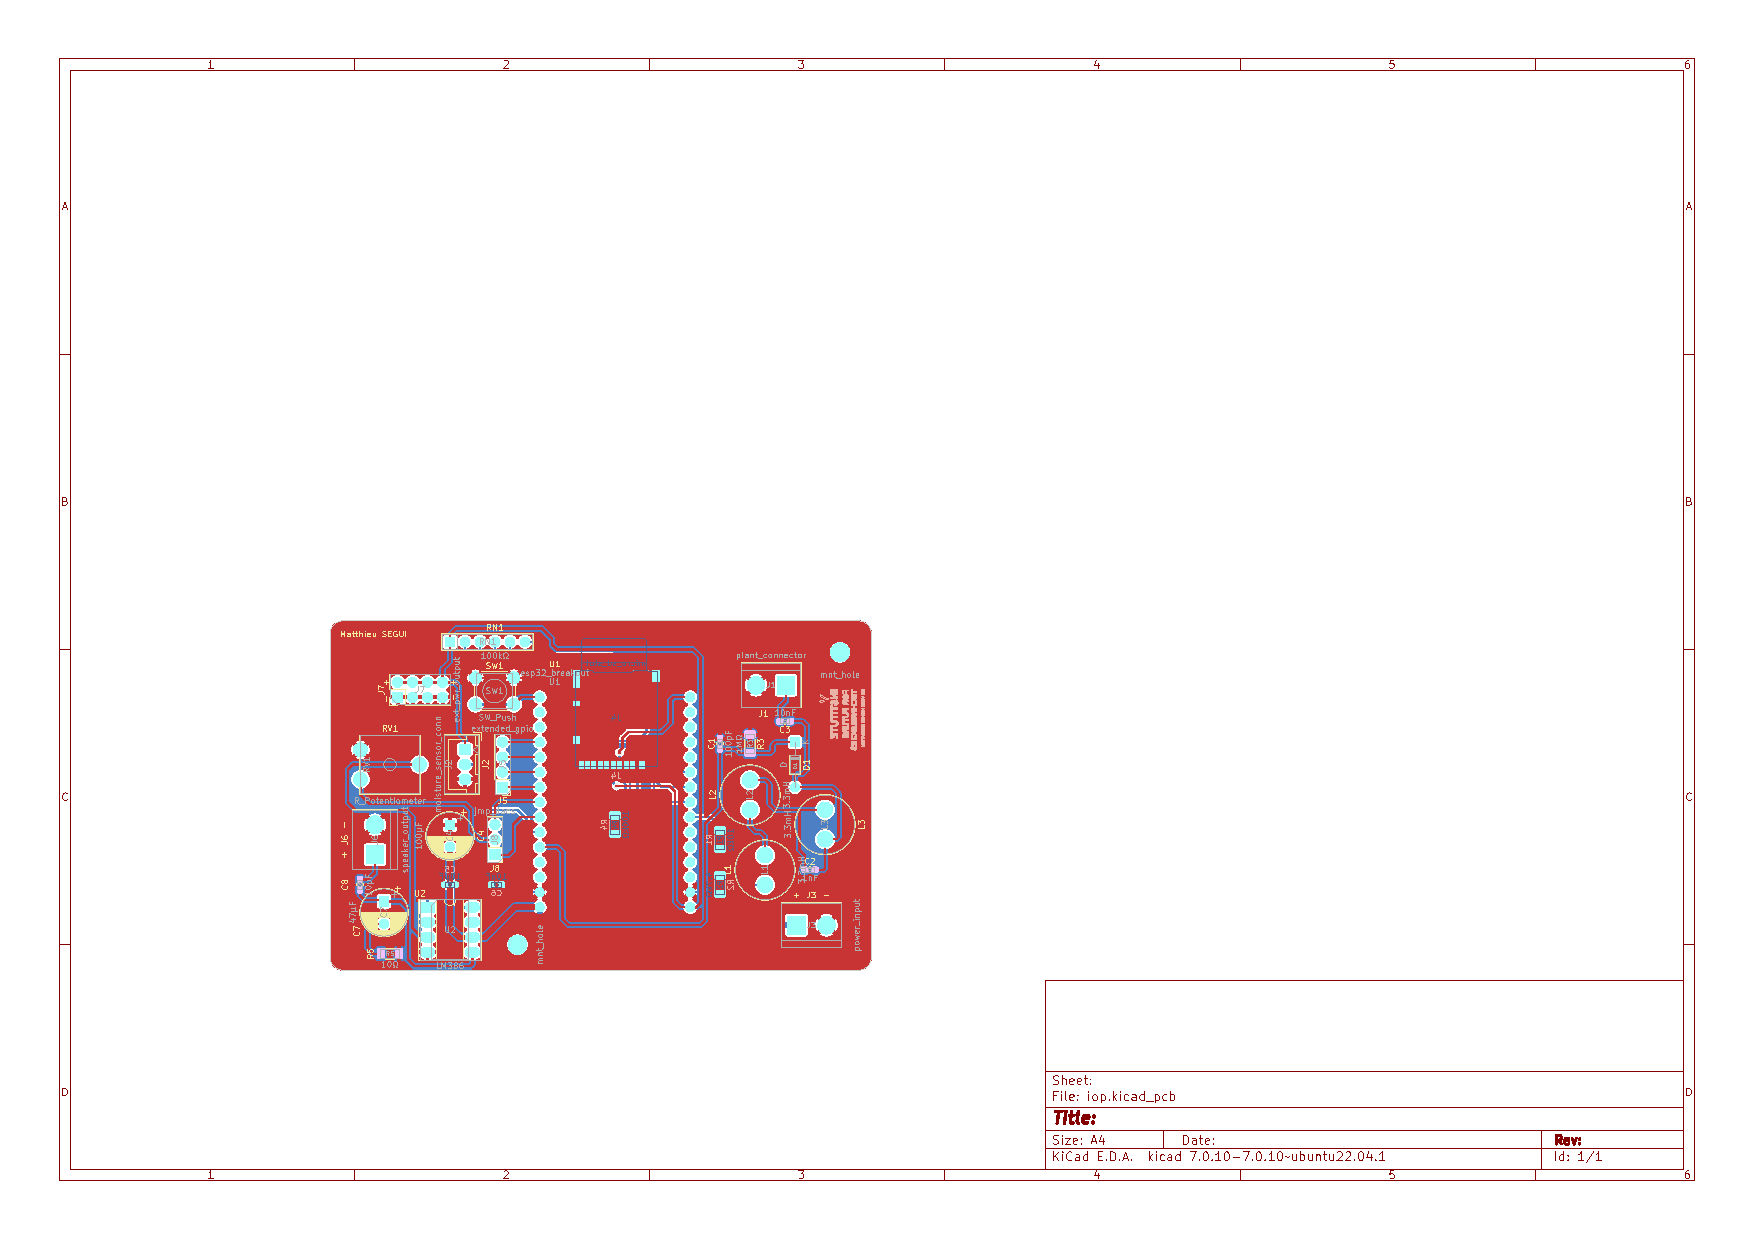
\includegraphics[width=\textwidth]{images/iop-routed_pcb.pdf}
    \caption{The routed double sided PCB.} 
    \vspace{0.1cm}
    \label{fig:iop_routed_pcb}
\end{figure}

Kicad also allows us to generated a 3D view of the future PCB. This allows us to imagine what the
PCB will look like when it will be manufactured.
\begin{figure}[h!]
    \centering
    \includegraphics[width=0.8\textwidth]{images/front_iop_3D_view_modified.png}
    \caption{Front 3D rendering of the built PCB. The rendering is done using open source software: Kicad} 
    \vspace{0.1cm}
    \label{fig:front_iop_3D_view_modified}
\end{figure}

\subsection{Human interaction}

The device is able to capture the human interaction with the plant. The touch interaction is inducing changes
in the impedance, capacitance and inductance of the plant. Values are captured.

\subsubsection{Sonification on the device}
\newpage
\subsubsection{User study}
\paragraph{Abstract of user study}
This study explores human-plant interaction.
This study has been conducted in order to understand what kind of interaction we have to detect in order to have the best and more natural kind of interaction with plants.
The results will be applied in the Internet of Plants (IoP) project which intends to create a fully connected bio-organ system.
The IoP is looking to reduce the gap between humans and plants by creating a symbiotic relationship between 
nature and technology. We envision a world where our daily objects are responsive.

\paragraph{Introduction}
Plants represent a full ecosystem of evolution, adaptation and communication.

In the context of the Internet of Plant (IoP) project, this study aims to extract the natural interaction between people and plants.
This experiment explores the interactions the IoP device will have to detect to create a symbiotic relation between human and plants. 
The physical touch is the starting point of a sonification process.
Sonification is “the use of non-speech audio to convey information or perceptualize data” \cite{kramer2010sonification}.
Three distinct plant species—\textit{Dypsis lutescens, Pachira glabra, and Dracaena}—are employed as subjects to extract user perceptions and interactions within this framework. 

The methodology engages students from the engineering school and two researchers.
The participants are asked to interact with the plants and imagine the sounds that could be generated by the plants.

The correlation between plant height and trunk interactions reveals environmental factors impacting human-plant dynamics.
Additionally, interactions are categorized based on intensity, spatial displacement, and duration.


\paragraph{Methodology}

\subparagraph{Participants}
The study is conducted on 22 participants. Participants are mainly composed of engineering students. The participant set includes 15 males and 7 females.
The age of participants is between 19 and 22 years old. Exception for three participants that are older than 22 years old. 




\subparagraph{The Procedure} 
We introduced the subject telling participants : 
"We're in the very near future. You are looking at plants that make music when you physically interact with them (it is not actually the case, but imagine it). Explore their capabilities."
Using this prompt, we tried not to bridle them to much but approach them to the physical interaction component.
Subsequently, participants were given time to explore the potential musical capacities of the plants at their own pace.
We conducted the study without providing any guidance during the exploration phase.
In instances where participants encountered difficulty initiating exploration, the prompt was reiterated to encourage the participants to explore.
This methodological approach was designed to capture the intuitive and natural human-plant interaction.
Also, we avoided any kind of communication or talking between 2 participants to reduce the potential bias.


\subparagraph{Materials/Tools}

To proceed and conduct this user study, we chose 3 different plants from 3 different species.


\textit{\textbf{Dracaena}}: It has long leaves and fragile perceived trunk but also flexible. The plant is 95 cm tall.

\begin{figure}[h!]
    \centering
    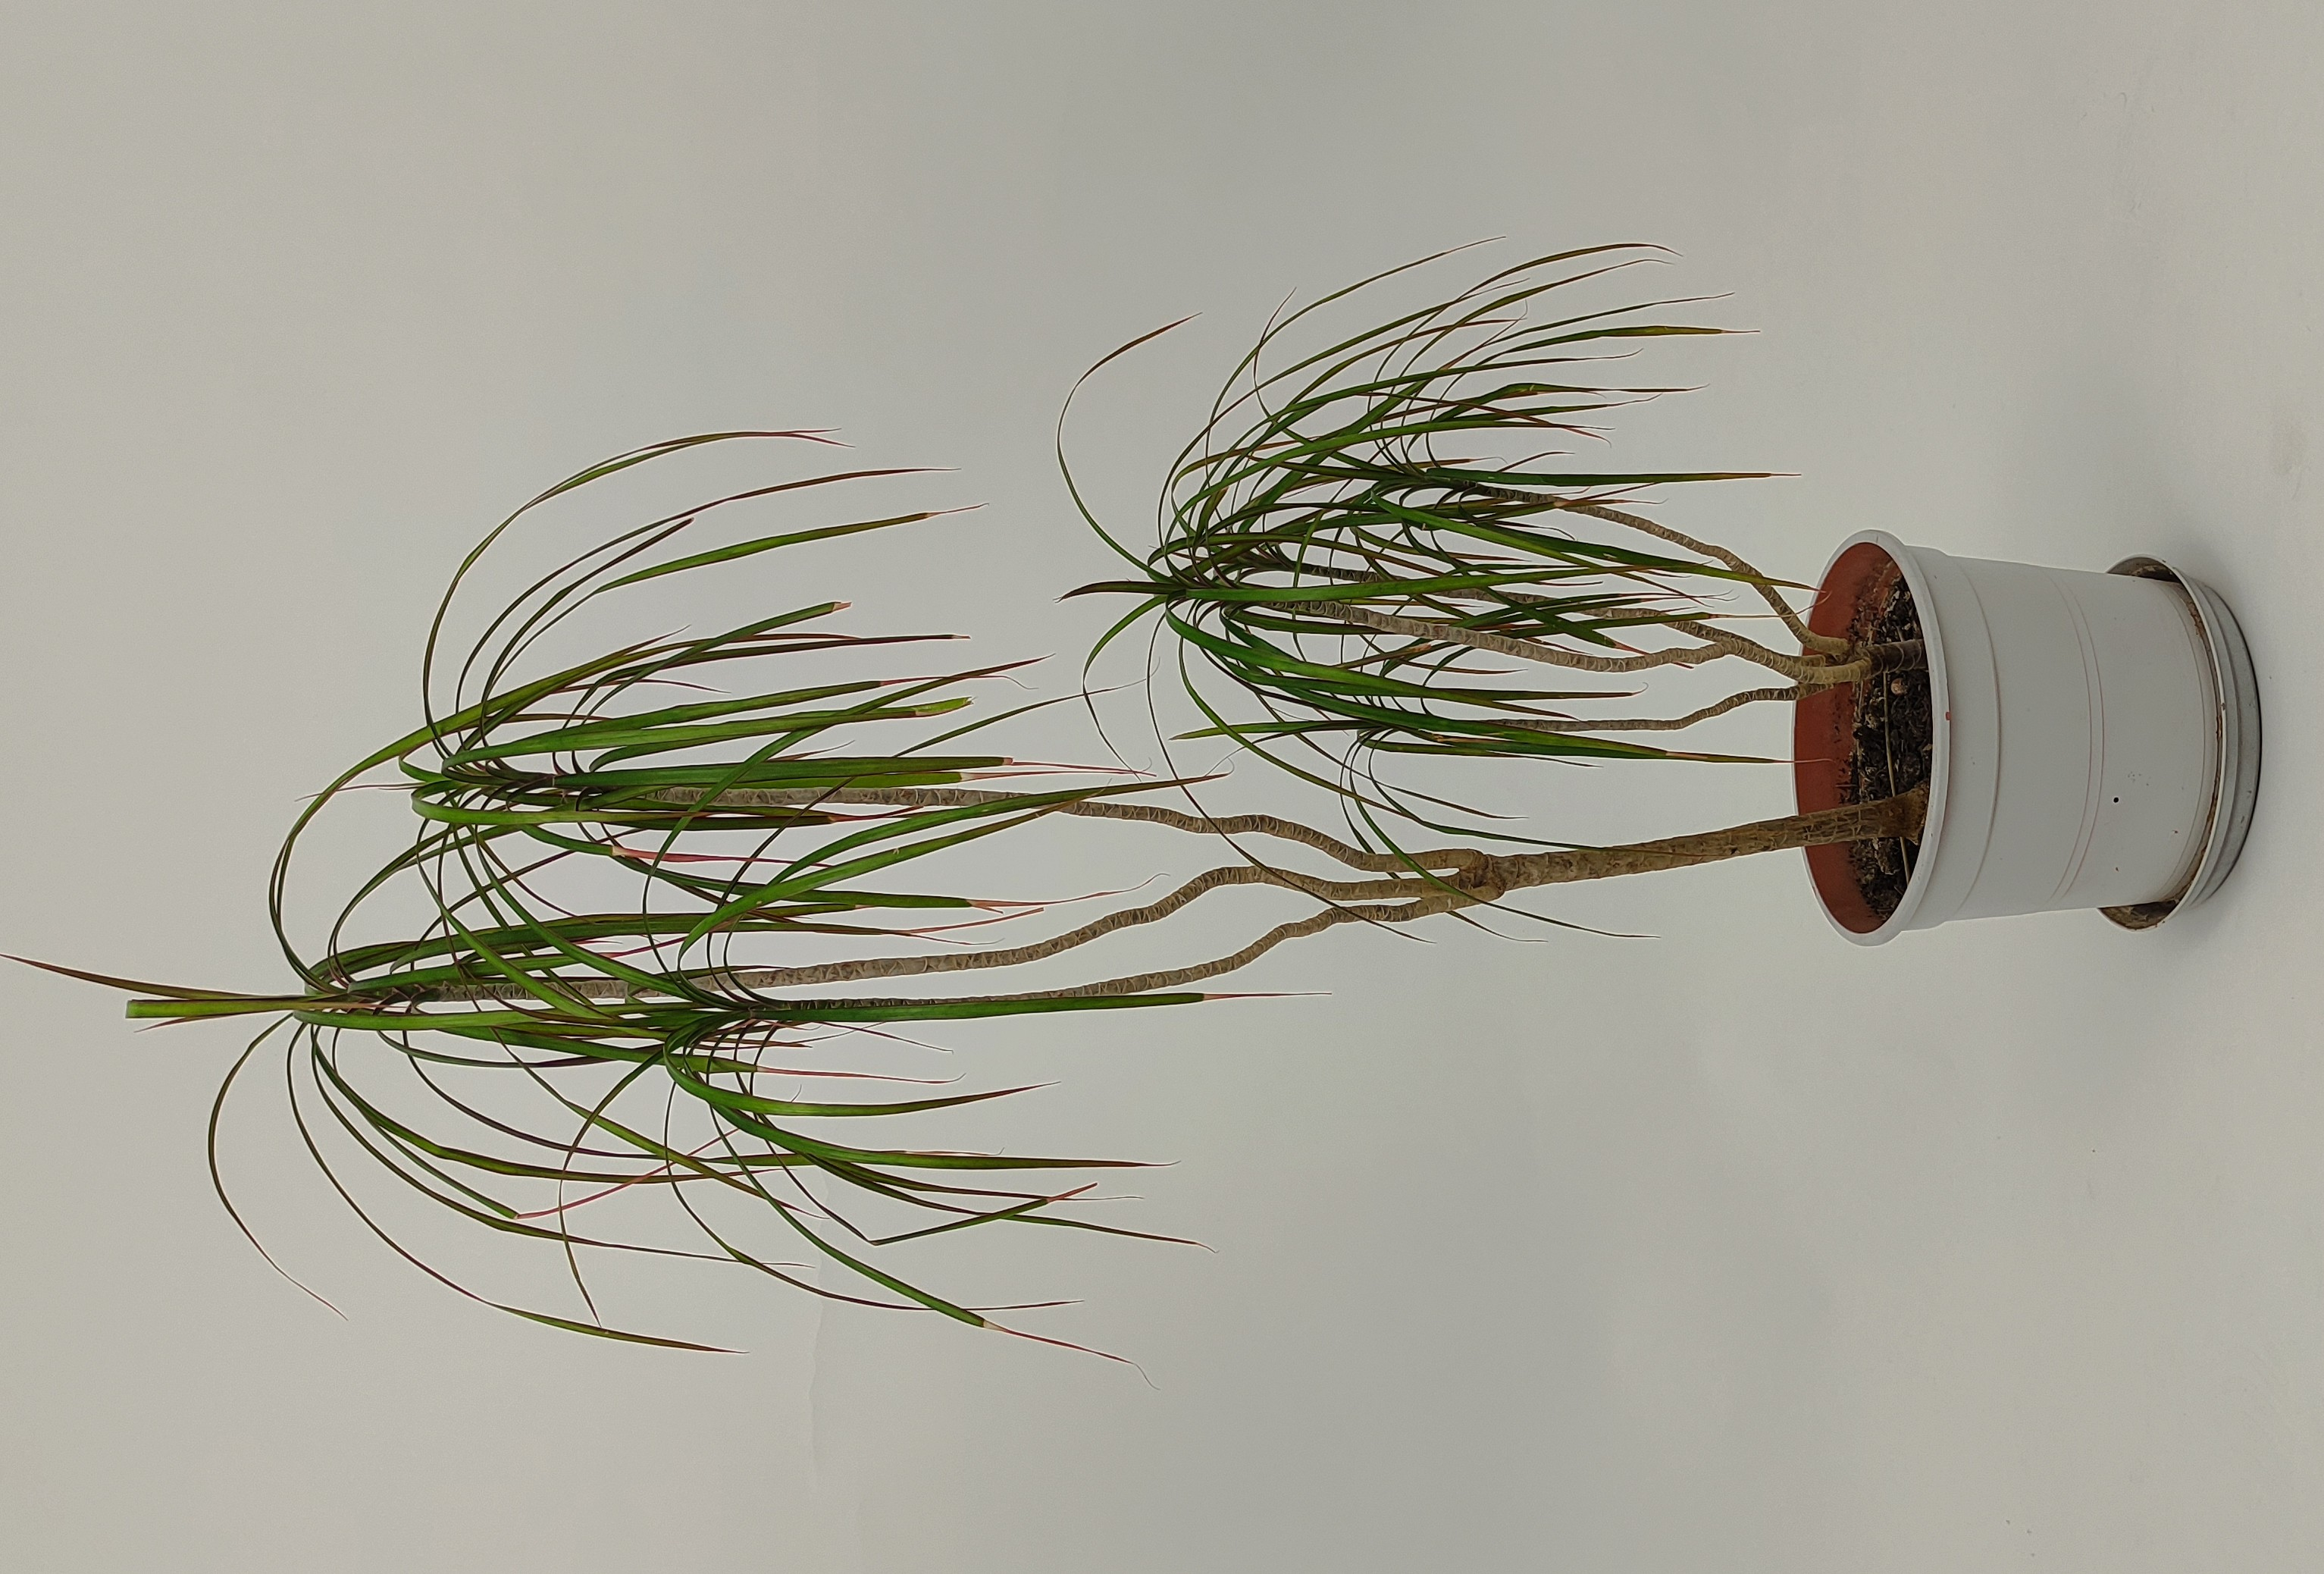
\includegraphics[width=0.8\textwidth, angle=-90]{small_plant.jpg}
    \caption{The N°1 plant is a \textit{Dracaena}.}
    
    \vspace{-0.5cm}
    \label{fig:small_plant}
    \vspace{0.2cm}
\end{figure}




\textit{\textbf{Pachira glabra}}:We chose to use this plant for its large leaves and its wide trunk.
The plant is 110 cm tall.

\begin{figure}[h!]
    \centering
    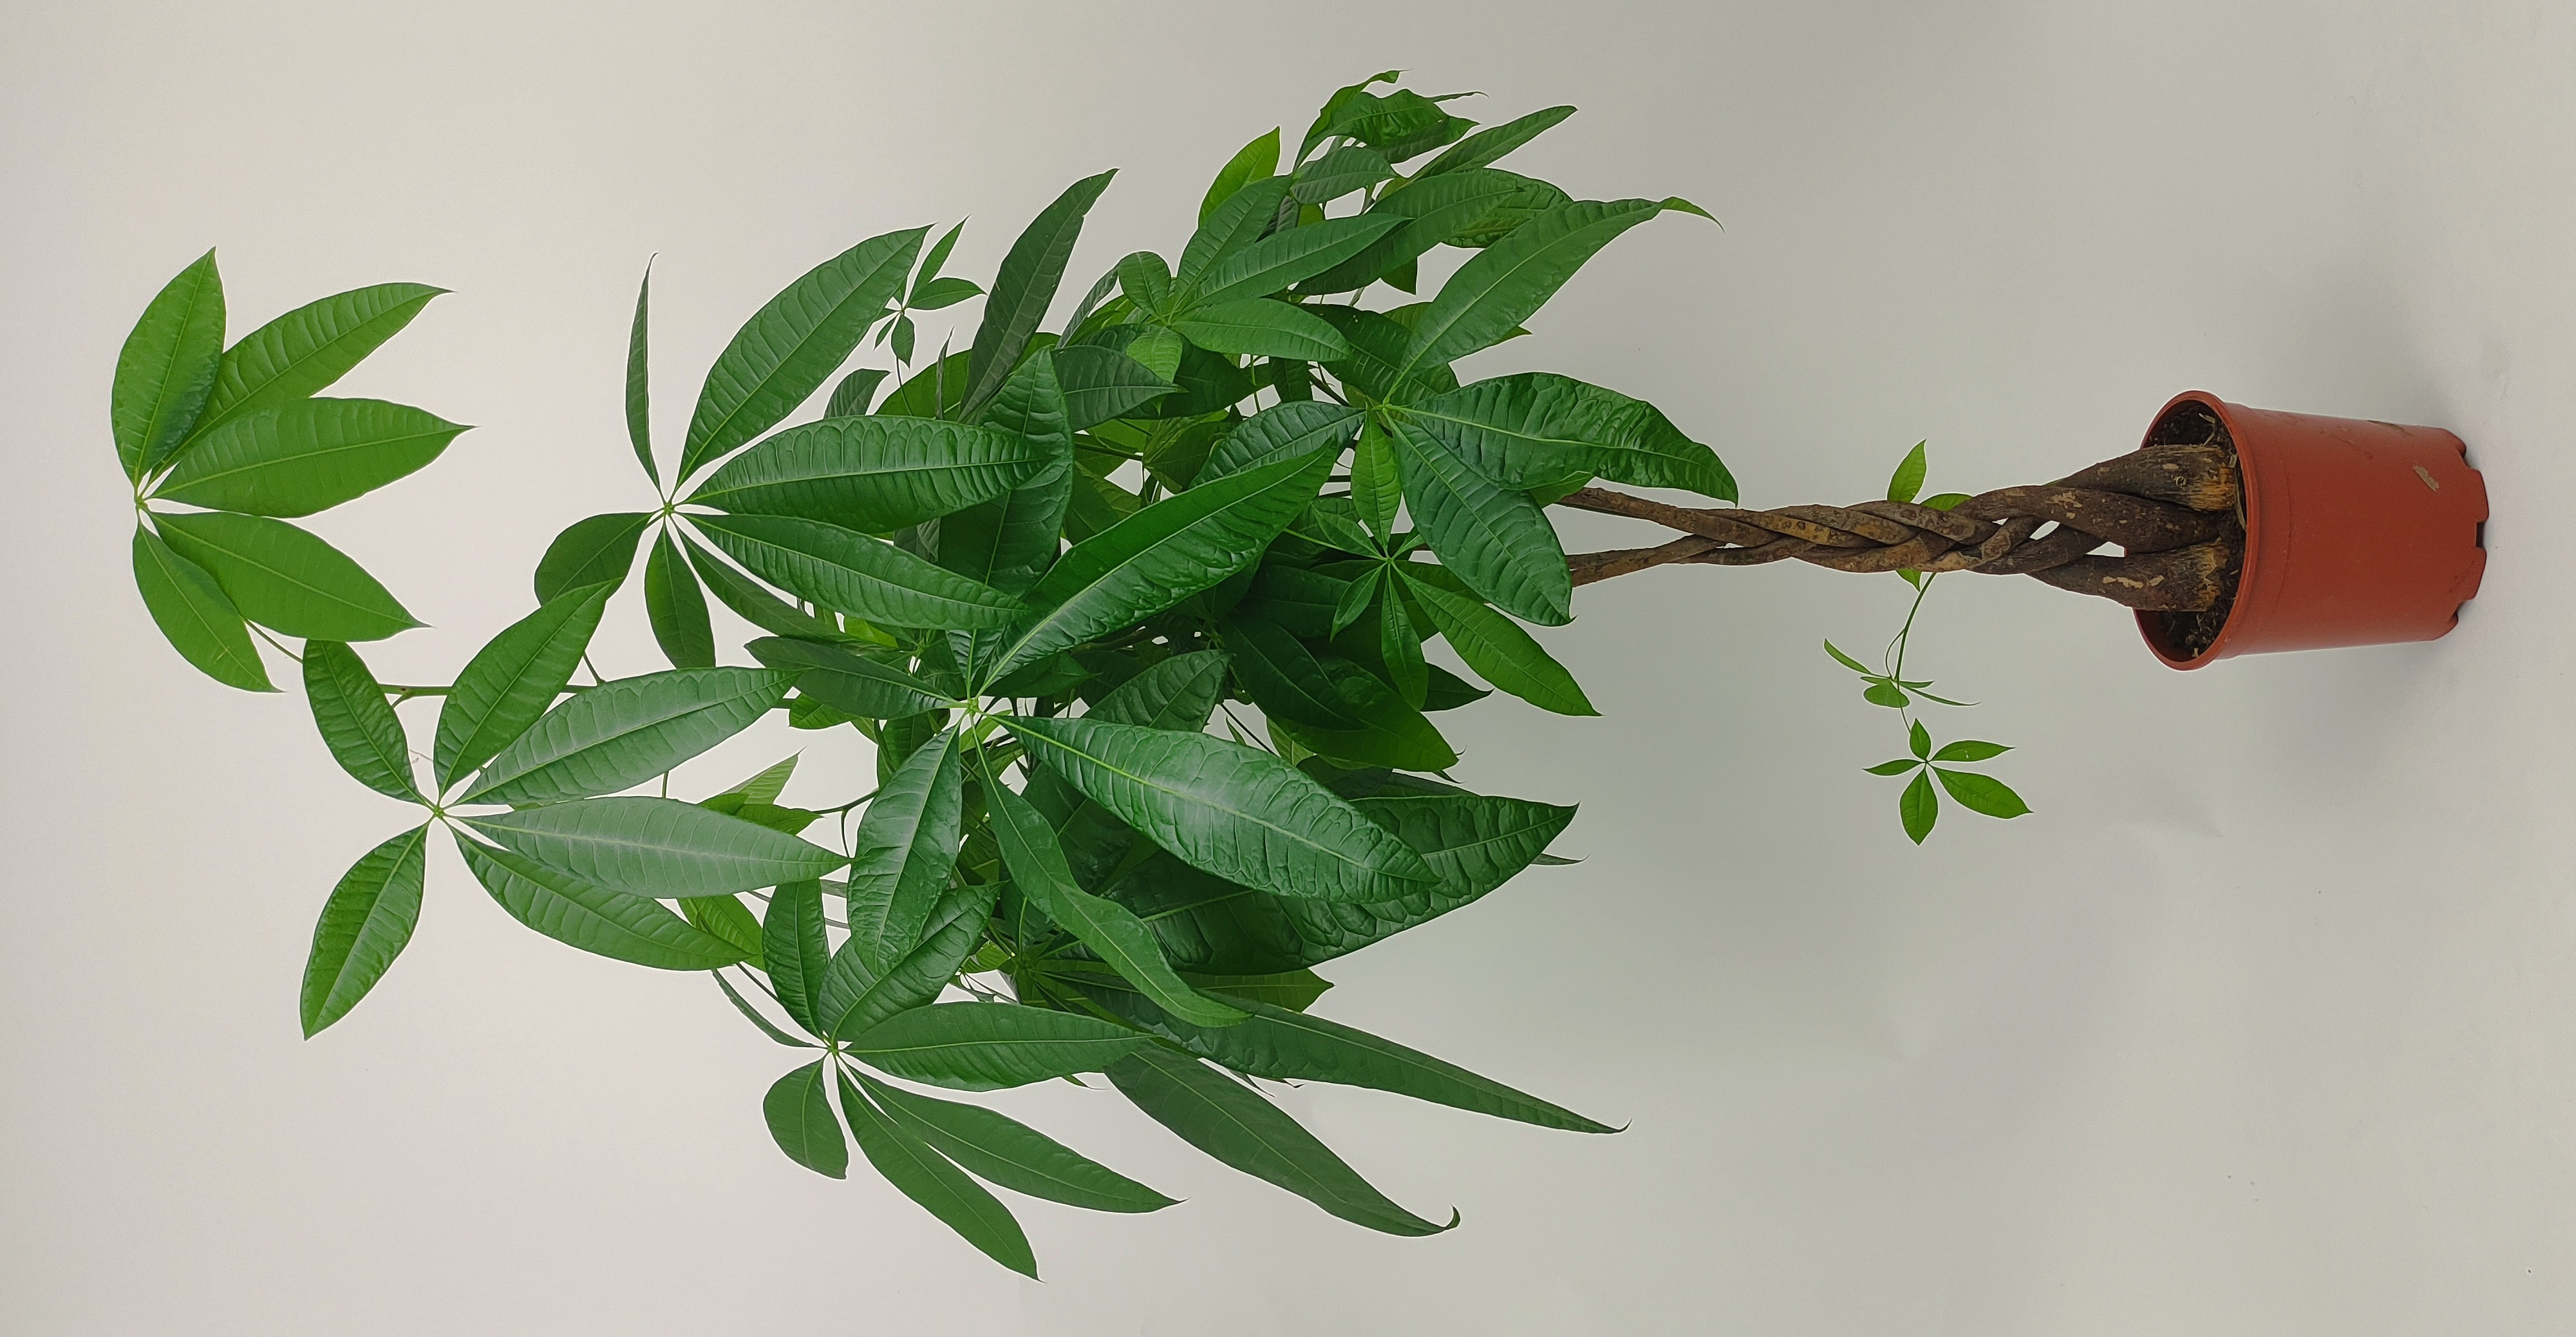
\includegraphics[width=0.8\textwidth, angle=-90]{tall_plant_cropped.jpg}
    \caption{The N°2 plant is a \textit{Pachira glabra}.}
    
    \vspace{-0.5cm}
    \label{fig:tall_plant}
    \vspace{0.2cm}
\end{figure}



\textit{\textbf{Dypsis lutescens}}: The \textit{Dypsis lutescens} is composed of many trunks and stems. On top of that, the leaves are numerous and tight. The plant is \hl{...} tall.

\begin{figure}[h!]
    \centering
    \includegraphics[width=0.8\textwidth, angle=-90]{fougere_plant.jpg}
    \caption{The N°3 plant is a \textit{Dypsis lutescens}.}
    
    \vspace{-0.5cm}
    \label{fig:fougere_plant}
    \vspace{0.2cm}
\end{figure}



\subparagraph*{The experimental space}
The experimental space featured three distinct levels of height, each corresponding to one of the three plants introduced to participants.

\begin{figure}[h]
    \centering
    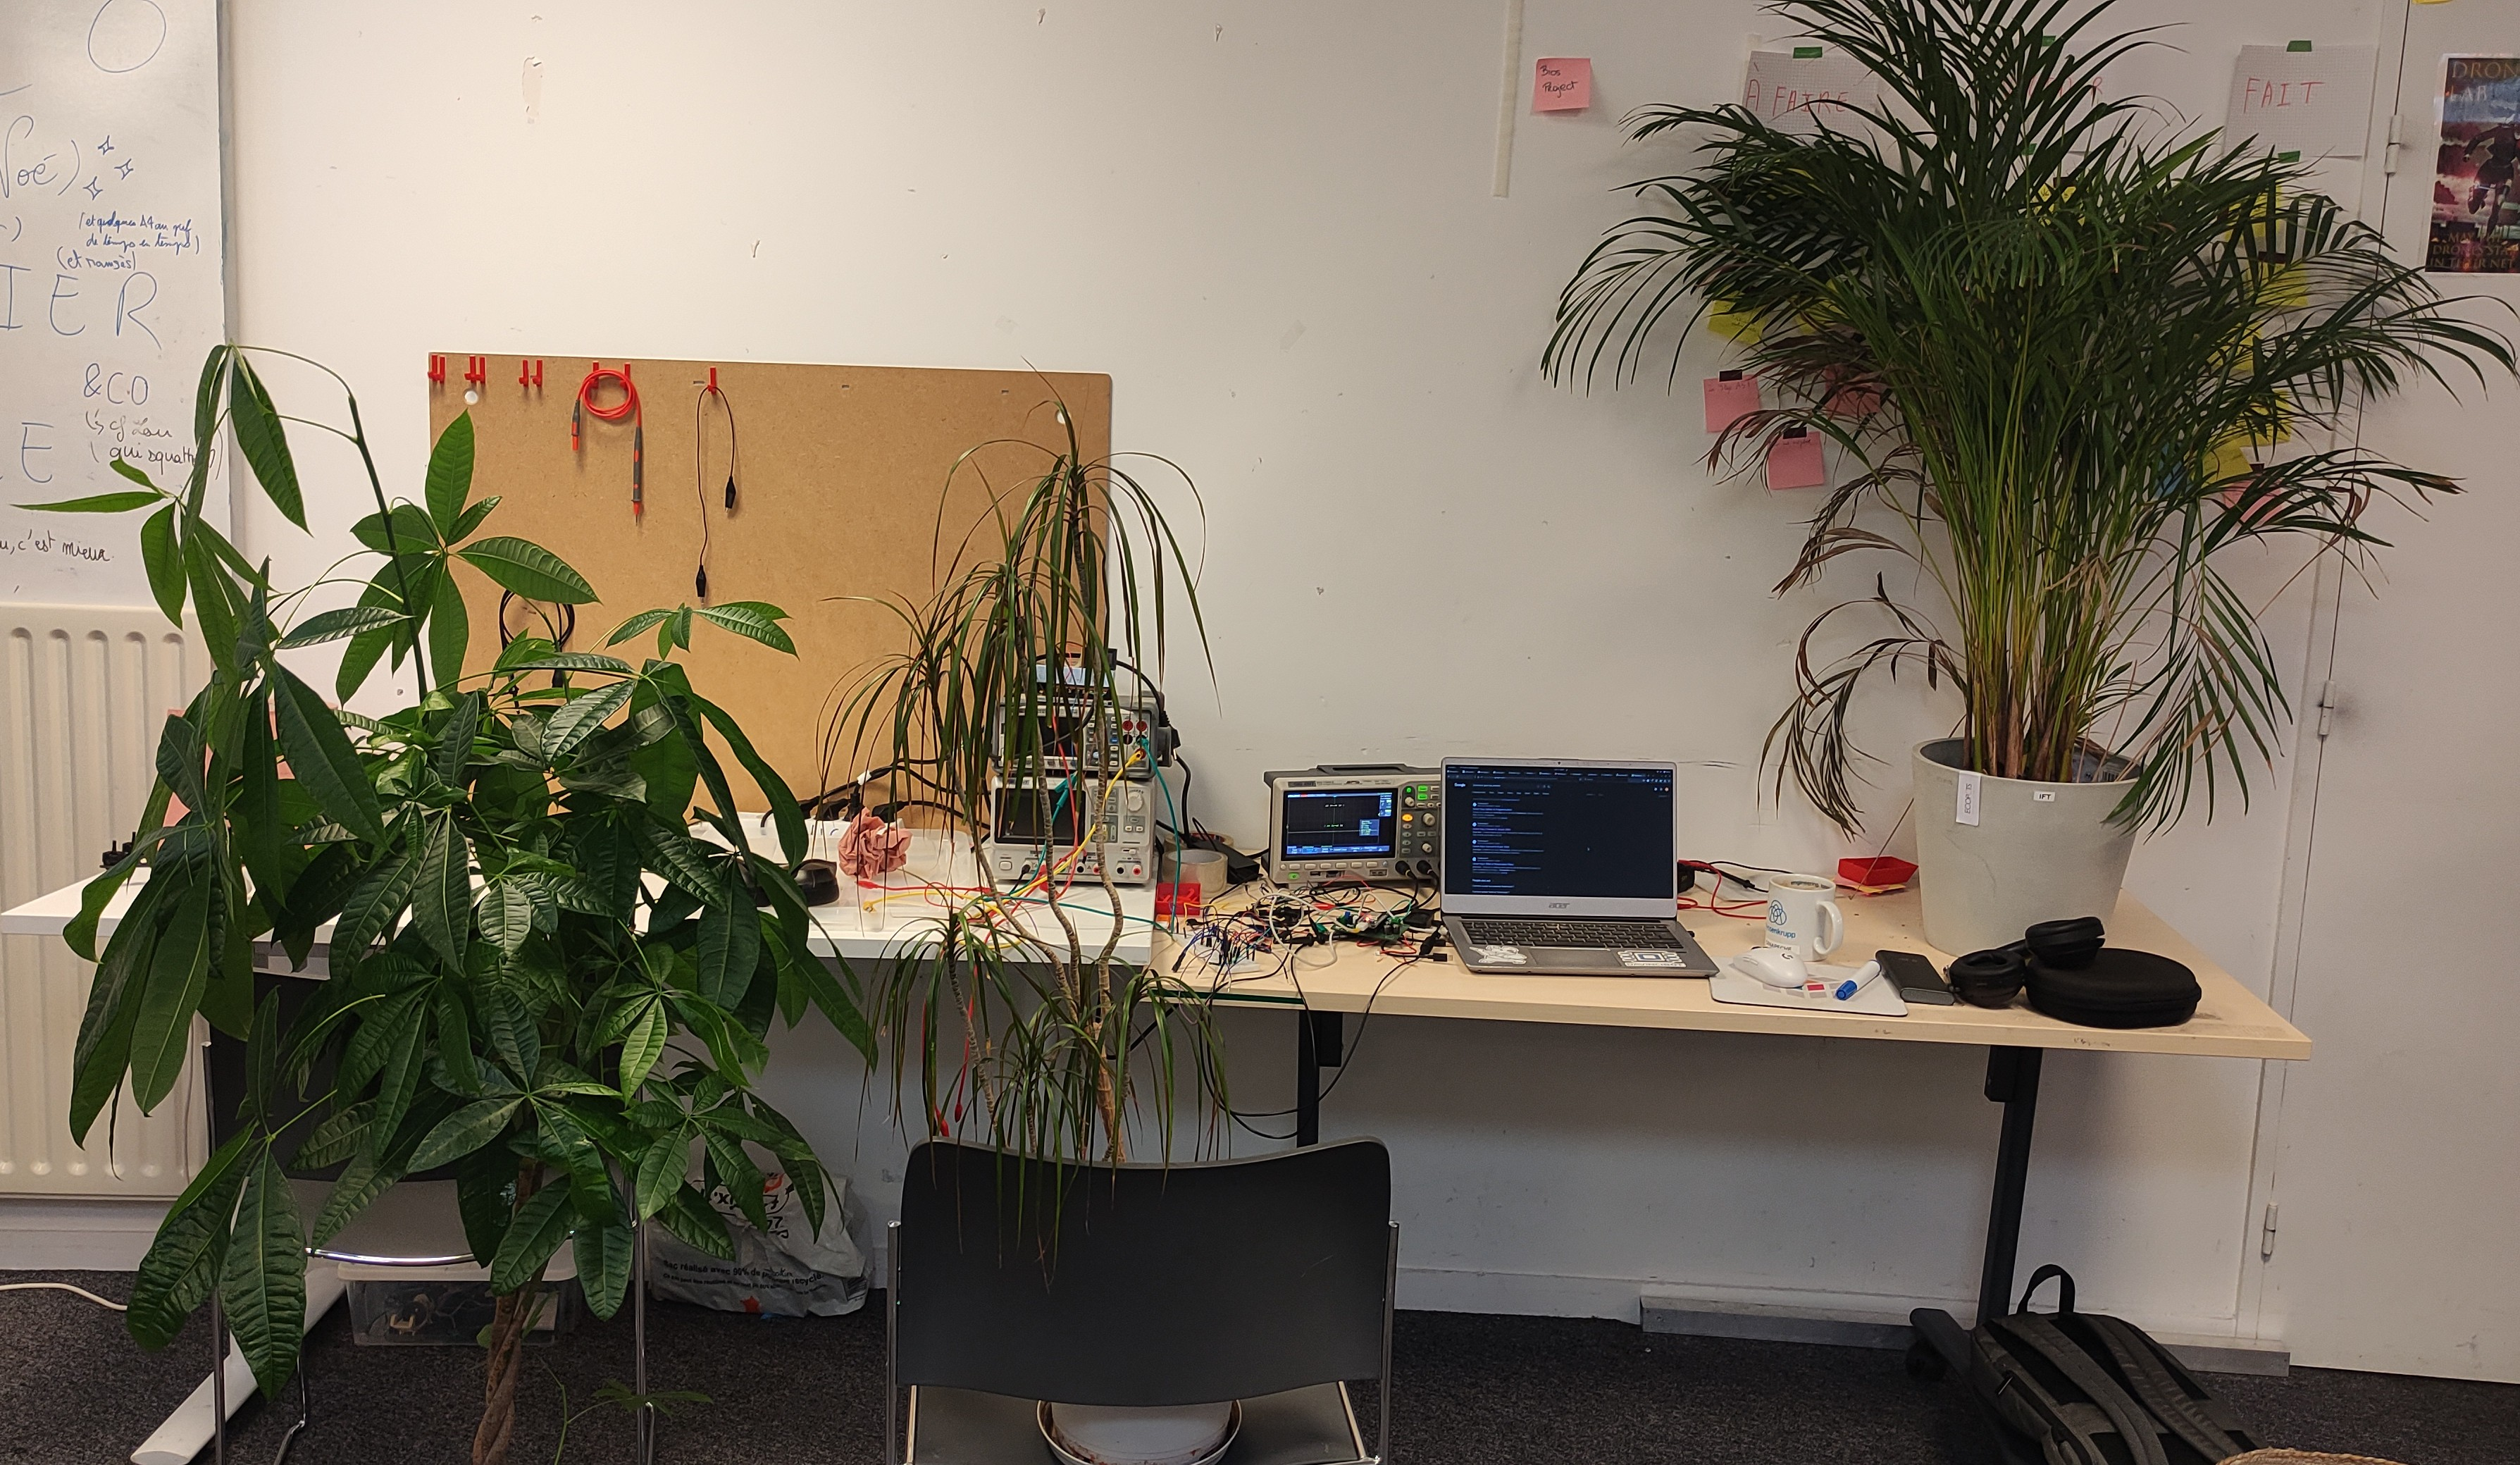
\includegraphics[width=0.8\textwidth]{setup_user_study.jpg}
    \caption{User study space setup. The setup is built from our lab space.}
    
    \vspace{-0.5cm}
    \label{fig:setup_user_study}
    \vspace{0.2cm}
\end{figure}

\paragraph{Data collection}
To capture the participant's interactions with the plants, a collaborative approach was adopted, involving two researchers to provide dual perspectives.
Throughout the exploration phase, both researchers took notes, documenting the diverse ways in which participants engaged with the three distinct plants.
The researchers explicitly specified the plant involved in the interaction in order to extract special features related to a specific plant.

The written notes retrieved descriptions of participants' actions, movements and interactions.
The dual-observer strategy tends to reduce the potential biased.

At the beginning of the experiment, the \textit{Dypsis lutescens} was on the floor, the \textit{Dracaena} was on a chair and the \textit{Pachira Glabra} was on a table.
At the middle of the experiment, we switched the \textit{Dypsis lutescens} and the \textit{Pachira Glabra} to see if the participants would interact differently with the plants.
The set-up of the experiment is shown in Figure \ref{fig:setup_user_study}. 


\paragraph{Results}

The data given by the user study allowed us to define 5 main types of interaction. Those interactions are defined by the way the user interacts with the plant. The 5 main types of interaction are :

\begin{itemize}
    \item Grasp : user uses the whole hand to grab trunk or leaves.
    \item Pinch : user uses 2 to 3 digits to grab trunk or leaves.
    \item Slide : user uses his/her hand or finger to slide on the plant whether is on a leave or on the trunk. The action is continuous.
    \item Pet : user uses his/her hand to cuddle the plant or to pass through the leaves. The user is moving his/her hand in space. She/he is not staying still or staying on a particular object.
    \item Tam Tam : user taps on the plant mainly using the whole hand.
\end{itemize}



Looking at the results, we extracted the table \ref{tab:results}.


\begin{table}[ht]
\begin{tabular}{|l|ll|l|ll|}
\hline
\multirow{2}{*}{Plant/Interaction} & \multicolumn{2}{l|}{Group 1}       & Group 2 & \multicolumn{2}{l|}{Group 3}       \\ \cline{2-6} 
                                   & \multicolumn{1}{l|}{Grasp} & Pinch & Slide   & \multicolumn{1}{l|}{Pet} & Tam Tam \\ \hline
Plant N°1                          & \multicolumn{1}{l|}{4}     & 8     & 4       & \multicolumn{1}{l|}{4}   & 2       \\ \hline
Plant N°2                          & \multicolumn{1}{l|}{9}     & 3     & 3       & \multicolumn{1}{l|}{3}   & 10      \\ \hline
Plant N°3                          & \multicolumn{1}{l|}{10}    & 1     & 5       & \multicolumn{1}{l|}{7}   & 3       \\ \hline
Total                              & \multicolumn{1}{l|}{23}    & 12    & 12      & \multicolumn{1}{l|}{14}  & 15      \\ \hline
\end{tabular}
% \caption*{Plant N°1 : Petite | Plant N°2 : Grande | Plant N°3 : Fougère}
\caption{Raw results extracted from the user study}
\label{tab:results}
\end{table}


With the extraction of the result we were able to design a bar chart.
The graph is grouping the interactions by plant. The height of the bar is the number of participants that performed the interaction.
The graph is shown in figure \ref{fig:setup_user_study}.


\begin{figure}[ht]
    \centering
    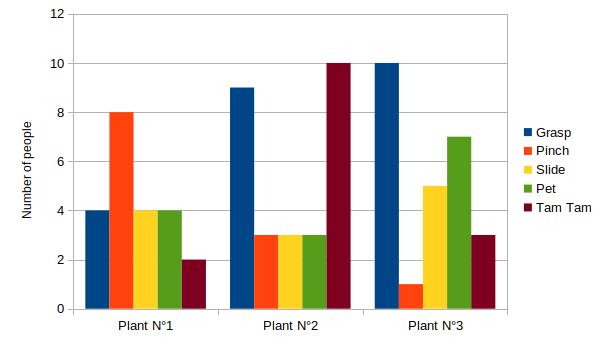
\includegraphics[width=\textwidth]{plant_interaction_chart_2.png}
    \caption{Bar chart that is extracting the main types of interaction regarding each plants.}
    
    \vspace{-0.5cm}
    \label{fig:chart_interaction}
    \vspace{0.2cm}
\end{figure}

In the end, of the 22 participants, 15 were already familiar with the project and 7 were not.

\paragraph{Discussion}
Looking at the results, the interaction were various depending on the plant. 
Thus, we can extract main interactions that are linked to the plant type. 
Looking at table \ref{tab:results}, people are more inclined to use their hands as tam tam or grasp the \textit{Pachira glabra}. 
However, for the \textit{Dracaena} users prefer to pinch the trunk or leave. 
Participants decided to grasp whether a pack of trunk or leaves when it came to \textit{Dypsis lutescens}.
This is induced by many factors including the leaves shape, the width of the trunk.


It was observed that when the plants were positioned at higher elevations on the table, individuals tended to engage more with the trunk of the plants.

Looking at table \ref{tab:results}, we decided to group interaction. This was done by grouping type of interaction depending on 3 main factors :

\begin{itemize}
    \item The intensity factor : what is the intensity of the interaction (ex : pinch is lighter than grasp)
    \item The spatial factor : what is the interaction displacement.
    \item The duration factor : what is the interaction duration (ex : tam tam is instantaneous).
\end{itemize}

The "Group 1" includes the pinch and grasp interaction. Indeed, looking at the 3 factors we defined, 
the pinch and grasp are high in intensity and long in duration but people stay still in space.
This group of interaction can be defined as \textbf{binary interaction}. The user is either grasping or not.

The "Group 2" includes the slide. The slide interaction is long in time, it moves in space but low in intensity.
This group of interaction can be defined as \textbf{continuous interaction}.


Whereas, the "Group 3" includes the pet and Tam Tam. 
These 2 interactions are really high in intensity, people usually tam tam and pet in different places but those interactions are short in time. 
This group is defined as \textbf{repetitive interaction}. The user is repeating the same action over and over again.


\begin{figure}

    \begin{minipage}{.5\linewidth}
    \centering
    \subfloat[]{
        \includegraphics[scale=.4]{group_1_int_dia.png}
        
        \label{fig:interactions:subfig:group1}
        }
    \end{minipage}%
    \begin{minipage}{.5\linewidth}
    \centering
    \subfloat[]{\label{fig:interactions:subfig:group2}\includegraphics[scale=.4]{group_2_int_dia.png}}
    \end{minipage}\par\medskip
    \centering
    \subfloat[]{\label{fig:interactions:subfig:group3}\includegraphics[scale=.4, width=0.5\textwidth]{group_3_int_dia.png}}
    
    \caption{Figure showing graphically the intensity of the 3 types of factors we defined. (a) Group 1 : pinch and grasp. (b) Group 2 : slide. (c) Group 3 : pet and tam tam.}
    \label{fig:main}
    \end{figure}


The participants we interviewed introduced a bias in the results.
They were all students from the engineering school and thus, they all had a similar background.
Some of them were already familiar with the project.

\paragraph{Conclusion}

During our study on the Internet of Plant project, we've captured insights into how people might interact with plants in a future where they make music through touch.

Our three chosen plants influenced how participants engaged with them. We observed everything from gentle petting to energetic drumming on the plants.
Interestingly, we found that when the plants were higher up, participants tended to focus more on the trunk.

By grouping interactions based on factors like intensity and duration, we gained a clearer picture of how people approached these musical plants.
It turns out that certain interactions, like grasping and pinching, were more common, while others, like sliding, had their own distinct appeal.

Regarding to the results we thought about what could be done with the defined interactions.
For instance, the sound generated from the interaction could be linked to the kind of interaction.
People doing Tam Tam on the plant will expect a drum sound. Whereas, people performing a slide will expect a sound closer to a continuous organ sound.
The possibilities are endless and the only restrictions are the capabilities of the device capturing the interaction. 
\subsection{...}